\documentclass[10pt,twocolumn]{article}
\usepackage[margin=0.68in]{geometry}
\usepackage{amsmath,amssymb,amsthm}
\usepackage{graphicx}
\usepackage{color}

\definecolor{navy}{RGB}{15, 23, 42}
\definecolor{accent}{RGB}{16, 185, 129}
\definecolor{blueacc}{RGB}{37, 99, 235}
\definecolor{softbg}{RGB}{241, 245, 249}
\definecolor{tealbg}{RGB}{236, 253, 245}

\makeatletter
\renewcommand\section{\@startsection{section}{1}{\z@}{-2.5ex \@plus -1ex \@minus -.2ex}{1.2ex \@plus .2ex}{\normalfont\large\bfseries\color{navy}}}
\renewcommand\subsection{\@startsection{subsection}{2}{\z@}{-2.0ex \@plus -0.5ex \@minus -.2ex}{0.8ex \@plus .2ex}{\normalfont\normalsize\bfseries\color{blueacc}}}
\makeatother

\newtheorem{proposition}{Proposition}
\newtheorem{theorem}{Theorem}
\newtheorem{remark}{Remark}

\title{\textbf{From Wavy Unitary Orbits to Trig-Free Cayley-Spinor Networks and Non-Abelian Sequence Memory}}
\author{Experimental Research Note \\ \texttt{clean-text-dataset} Workspace}
\date{November 16, 2026}

\begin{document}
\raggedbottom
\twocolumn[
\begin{center}
{\LARGE\bfseries\color{navy} From Wavy Unitary Orbits to Trig-Free Cayley-Spinor Networks and Non-Abelian Sequence Memory}
\par\vspace{0.5em}
{\color{accent}\rule{0.35\textwidth}{1.5pt}}
\par\vspace{0.4em}
{\small\color{navy} \textbf{shu195} \quad$\bullet$\quad \texttt{github.com/shu195/cayley-spinor-networks} \quad$\bullet$\quad November 16, 2026}
\end{center}
\vspace{0.4em}
\noindent\colorbox{softbg}{\parbox{\dimexpr\textwidth-2\fboxsep\relax}{%
\small\textbf{\color{navy}Abstract.}
We trace a systematic experimental progression from complex-valued $U(1)$ phase-only neurons to non-abelian $SU(2)$ Cayley-Spinor architectures. Starting from a single $U(1)$ neuron, we first examine Bohr-like discrete amplitude shells trained via Straight-Through Estimation (STE), observing clean convergence on a single neuron ($3.11\times 10^{-8}$ MSE) but severe boundary chattering in multi-layer networks ($0.5397$ vs.\ $0.1627$ float MSE). Replacing discrete shells with a $C^\infty$ wavy polar surface $r(\theta) = r_0 + A\cos(n\theta + \phi)$ eliminates STE chattering, outperforms unconstrained complex float weights on an 8--16--4 network ($0.1525$ vs.\ $0.1627$) with half the per-weight parameters, and exhibits natural zero-crossing sparsity in recurrent graphs (75\% edge pruning with only $0.35\%$ MSE degradation on 16-node denoising). Extending this geometry to 4D quaternions ($S^3$), recurrent 32-node holographic recall, and finally a quantum-mechanical (QM) atom neuron model, we show that non-commuting operators eliminate the need for scalar activation functions. Crucially, we derive a trig-free rational Cayley Bloch-vector formulation of the $SU(2)$ spinor neuron requiring zero \texttt{sqrt}, \texttt{sin}, or \texttt{cos} evaluations while preserving exact unitarity ($\|\mathbf{e}\|_2 = 1$ to $3.33\times 10^{-16}$). Finally, we apply this Cayley $SU(2)$ map to associative sequence memory (\textit{QuatScan}): on an order-sensitive token task ($\text{pos}(A) < \text{pos}(B)$, $L=16$, zero positional encodings), commutative $U(1)$ memory is bounded at $53.5\%$, whereas Cayley $SU(2)$ memory with near-identity initialization ($\sigma_{\text{init}}=0.1$) achieves $100.0\%$ test accuracy with 65 total parameters and $|q_t|=1$ to $1.55\times 10^{-15}$.
}}
\vspace{1.0em}
]

\section{Introduction}
Standard neural networks separate linear mixing ($Wx + b$) from elementwise scalar nonlinearities ($\text{ReLU}, \tanh$). While hardware-friendly, this separation ignores phase interference, norm preservation, and non-commutative group structure. In this work, we investigate what happens when weights and hidden states are constrained to unitary and hypercomplex manifolds—and how to simplify the resulting equations so they run efficiently on standard silicon.

Our experiments uncover a sequence of concrete architectural insights and failure modes:
\begin{enumerate}
    \item \textbf{Single-$U(1)$ gauge degeneracy:} On a single input, $U(1)$ phase weights exhibit continuous gauge freedom; multi-sample batches collapse the degeneracy to machine precision ($3.86\times 10^{-17}$ MSE).
    \item \textbf{Bohr shells vs.\ wavy orbits:} Discrete radial shells suffer from STE boundary chattering at depth, whereas a smooth polar wave $r(\theta)$ restores $C^\infty$ gradients and induces natural sparsity.
    \item \textbf{Non-commuting QM atom neurons:} A single 4-orbital Schrödinger neuron $e^{-iH(x)}$ solves 2D XOR to $0.00000000$ MSE with zero activation functions.
    \item \textbf{Rational Cayley $SU(2)$ simplification:} An exact algebraic identity removes all eigendecompositions and trigonometric calls from $SU(2)$ Bloch rotations.
    \item \textbf{Non-abelian sequence memory:} Associative quaternion updates $q_t = u_t \otimes q_{t-1}$ solve order-sensitive tasks without positional encodings, provided near-identity initialization prevents random-walk scrambling on $S^3$.
\end{enumerate}

\begin{figure*}[t]
    \centering
    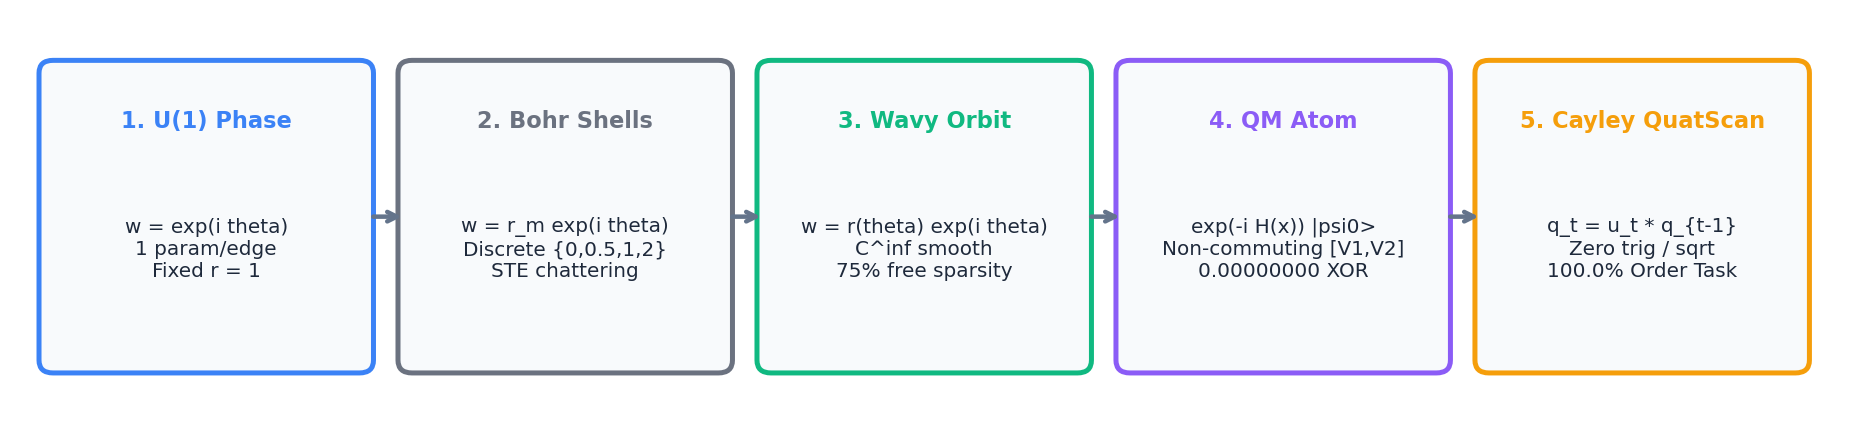
\includegraphics[width=0.96\textwidth]{figures/fig5_architecture_flow.png}
    \caption{Architectural progression from commutative $U(1)$ phase neurons to trig-free non-abelian Cayley-Spinor sequence memory.}
    \label{fig:arch_flow}
\end{figure*}

\section{Complex, Bohr-Shell, and Wavy-Orbit Neurons}

\subsection{Unitary $U(1)$ Phase Interference}
A $U(1)$-constrained complex neuron computes
\begin{equation}
    z = \sum_{k=1}^{d} e^{i\theta_k} x_k, \qquad \theta_k \in \mathbb{R},
\end{equation}
where each weight has exact unit modulus $|w_k| = 1$. Using Wirtinger calculus under $\mathcal{L} = \frac{1}{2}|z - y|^2$, the exact phase gradient is
\begin{equation}
    \frac{\partial \mathcal{L}}{\partial \theta_k} = \operatorname{Re}\!\left((z - y)^*\, i\, e^{i\theta_k} x_k\right).
\end{equation}
On a 1-neuron, 2-input verification, analytical gradients matched finite differences ($\epsilon = 10^{-7}$) to $1.57\times 10^{-10}$. On a single sample, the neuron converged to $6.26\times 10^{-6}$ MSE at $\theta = [0.8984, -0.3221]$ rather than the planted $[1.2, -0.7]$ due to a 1-DOF interference degeneracy; on a 4-sample linearly independent batch, it converged to $[1.2, -0.7]$ at $3.86\times 10^{-17}$ MSE.

Because Liouville's theorem forbids non-constant bounded entire activations on $\mathbb{C}$, we use the phase-preserving radial gate
\begin{equation}
    \operatorname{modReLU}(z; b) = \operatorname{ReLU}(|z| + b)\,\frac{z}{|z|}.
\end{equation}
On 4 samples with target $b=-1.2$, $\operatorname{modReLU}$ stalled at $0.00884$ MSE due to dead-zone regions ($|z|+b \le 0$).

\subsection{Bohr Discrete Shells and STE Chattering}
To allow amplitude attenuation without continuous float radii, we tested Bohr-inspired quantized shells $r_k \in \{0.0, 0.5, 1.0, 2.0\}$ with continuous latent $\rho_k$ updated via Straight-Through Estimation (STE):
\begin{equation}
    w_k = \operatorname{snap}(\rho_k)\, e^{i\theta_k}.
\end{equation}
On a 1-neuron target ($r=[2.0, 0.5]$), STE snapped exactly onto $[2.0, 0.5]$ with $3.11\times 10^{-8}$ MSE, whereas fixed-$U(1)$ stalled at $0.3614$. However, scaling to an 8--16--4 network (128 train / 64 test, 400 steps, $\text{lr}=0.05$) revealed severe STE boundary chattering: when $\rho$ crosses a midpoint ($0.75$ or $1.5$), discontinuous jumps in $|W|$ destabilize downstream phase interference.

\subsection{Smooth Wavy-Orbit Surfaces}
Replacing discrete shells with a smooth $n$-lobe polar curve eliminates STE entirely:
\begin{equation}
    w_k = r(\theta_k)\,e^{i\theta_k}, \qquad r(\theta) = r_0 + A\cos(n\theta + \phi),
\end{equation}
with $(r_0, A, \phi)$ shared per layer (still 1 learnable scalar $\theta_k$ per edge). Its derivative is $C^\infty$:
\begin{equation}
    \frac{\partial w_k}{\partial \theta_k} = \left(r'(\theta_k) + i\,r(\theta_k)\right)e^{i\theta_k}.
\end{equation}

\begin{table}[t]
\centering
\caption{8--16--4 Complex Network Benchmark (400 steps).}
\label{tab:8_16_4}
\begin{tabular}{lcc}
\hline
Model & Test MSE & Params/Weight \\
\hline
Bohr Shells + STE & $0.539732$ & $1 + 2\text{ bits}$ \\
Fixed $U(1)$ ($r=1$) & $0.262644$ & $1$ \\
Unconstrained Float & $0.162708$ & $2$ \\
\textbf{Wavy Orbit ($n=3$)} & $\mathbf{0.152465}$ & $\mathbf{1}$ \\
\hline
\end{tabular}
\end{table}

As shown in Table~\ref{tab:8_16_4}, the 3-lobe wavy orbit beat even unconstrained float weights ($0.1525$ vs.\ $0.1627$). In Layer~1, the optimizer learned $r_0=0.614, A=1.020$: because $A > r_0$, the orbit passes through zero at the troughs, acting as smooth, differentiable pruning.

\begin{figure}[t]
    \centering
    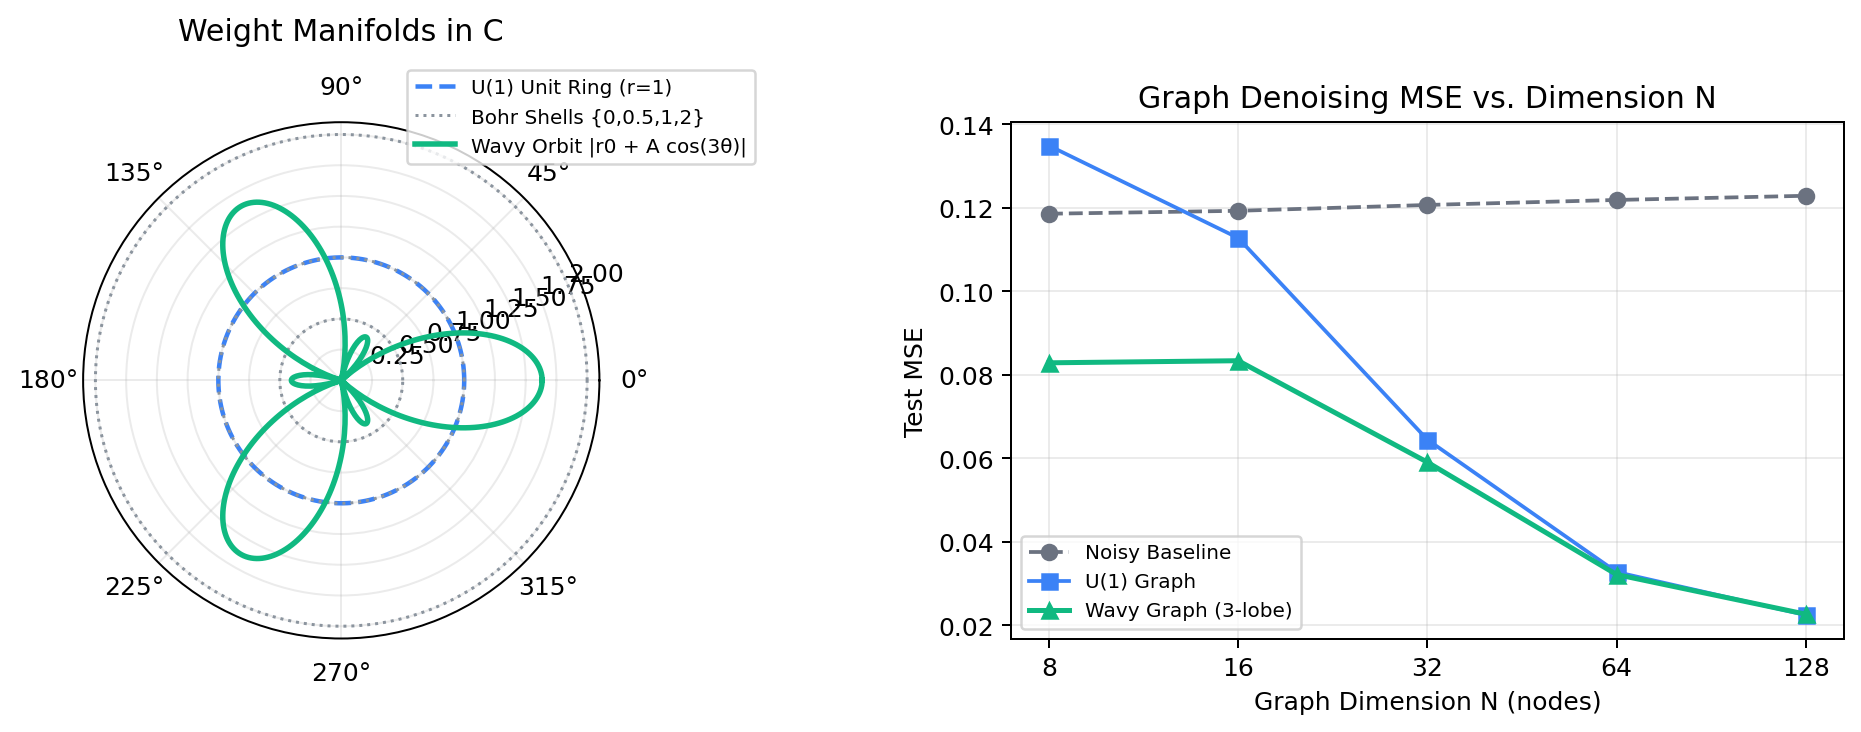
\includegraphics[width=\linewidth]{figures/fig1_bohr_wavy.png}
    \caption{Left: Comparison of $U(1)$, Bohr shells, and the learned 3-lobe wavy orbit in $\mathbb{C}$. Right: Graph denoising MSE vs.\ node dimension $N \in \{8,16,32,64,128\}$.}
    \label{fig:bohr_wavy}
\end{figure}

In a 3-layer 32--64--32--8 benchmark (600 steps, fan-in scaled), \texttt{wavy} ($4{,}457$ params) cut \texttt{u1} ($4{,}448$ params) error by more than $2\times$ ($0.5949$ vs.\ $1.2416$), while unconstrained \texttt{float} ($8{,}800$ params) reached $0.0069$ because the teacher had independent per-edge amplitudes.

\section{Graph-Coupled Wave Resonance and 4D Quaternions}

\subsection{All-to-All Resonant Graphs and Dimension Scaling}
Placing $N$ complex neurons on an all-to-all graph with $T$-step damped relaxation,
\begin{equation}
    z^{(t+1)} = (1 - \alpha) z^{(t)} + \alpha\,\operatorname{modReLU}\!\left(z^{(t)} W + \gamma X_{\text{in}},\, b\right),
\end{equation}
turns the network into a resonant cavity. On 16-node 3-mode wave denoising ($T=5$), \texttt{wavy} achieved $0.069346$ MSE vs.\ $0.088341$ (\texttt{u1}) and $0.122871$ (noisy baseline). Post-training magnitude pruning kept MSE nearly flat even after dropping $75\%$ of edges ($0.069346 \to 0.069590$, a $0.35\%$ shift).

Scaling $N \in \{8, 16, 32, 64, 128\}$ (Fig.~\ref{fig:bohr_wavy}, right) required normalizing shared wave gradients by $N^2$ (\texttt{np.mean} rather than \texttt{np.sum}) to prevent $\mathcal{O}(N^2)$ overflow. At low $N$, \texttt{wavy} strongly outperformed \texttt{u1} ($0.0829$ vs.\ $0.1349$ at $N=8$); as $N$ grew to $128$, both converged to $\approx 0.0226$ because $N^2$ pure phase edges already span the fixed $K=3$ signal subspace.

\begin{figure}[t]
    \centering
    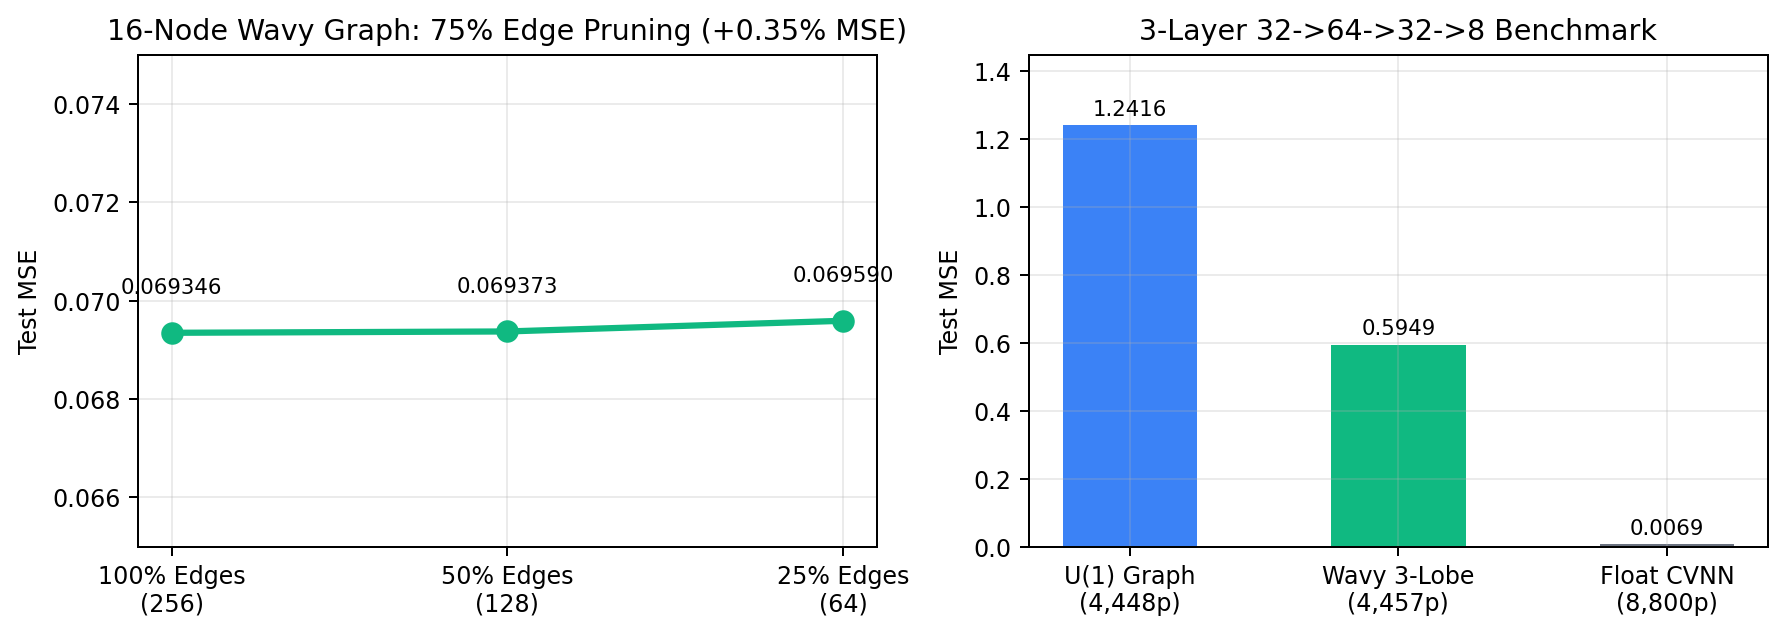
\includegraphics[width=\linewidth]{figures/fig6_pruning_and_3layer.png}
    \caption{Left: 16-node wavy graph holds flat MSE under 75\% edge pruning. Right: 3-layer 32--64--32--8 benchmark.}
    \label{fig:pruning_3layer}
\end{figure}

\subsection{32-Node Holographic Recall and Gauge Equivariance}
On a harder 32-node task where $50\%$ of input nodes were zeroed and corrupted with $0.35$ complex noise, we compared per-neuron 2-harmonic orbital cavities ($n_1=3, n_2=6$) against `u1` and a $4\times$-larger real $\tanh$ graph under both standard and unseen global phase-rotated ($\text{rot\_MSE}$, $X \mapsto e^{i\psi}X$) evaluation (Table~\ref{tab:holo}, Fig.~\ref{fig:holo}).

\begin{table}[t]
\centering
\small
\setlength{\tabcolsep}{3.5pt}
\caption{32-Node Holographic Recall (50\% wiped + 0.35 noise).}
\label{tab:holo}
\begin{tabular}{lcccc}
\hline
Model & Params & MSE & Phase & $\text{rot\_MSE}$ \\
\hline
Corrupted Input & $0$ & $0.4697$ & $0.445$ & $0.4697$ \\
Real $\tanh$ Graph & $4{,}160$ & $\mathbf{0.1461}$ & $\mathbf{0.862}$ & $0.7206$ \\
$U(1)$ Graph & $1{,}088$ & $0.2099$ & $0.801$ & $0.2099$ \\
\textbf{Harmonic Orbital} & $1{,}248$ & $0.1590$ & $0.856$ & $\mathbf{0.1590}$ \\
\hline
\end{tabular}
\end{table}

\begin{figure}[t]
    \centering
    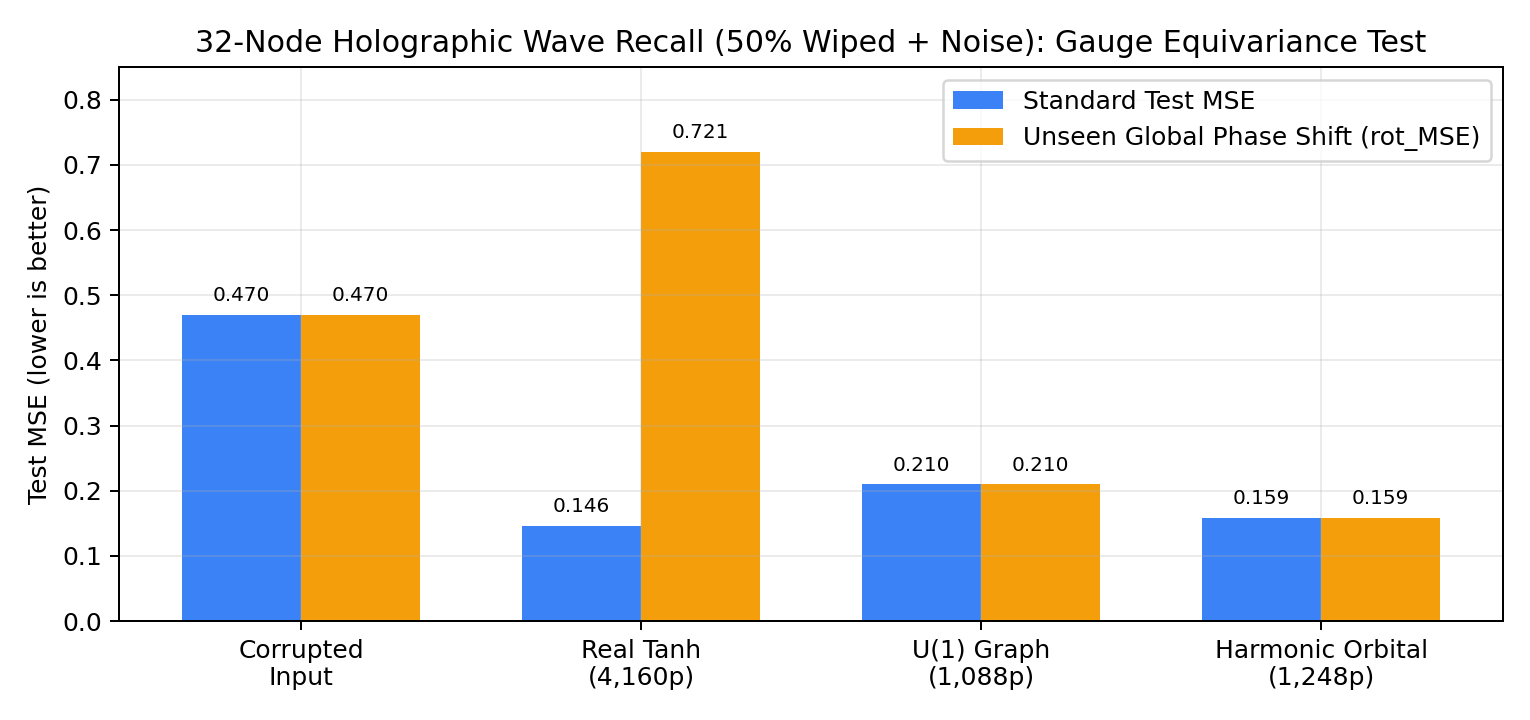
\includegraphics[width=\linewidth]{figures/fig2_holographic_recall.png}
    \caption{Real $\tanh$ memorizes absolute coordinates and collapses under unseen global phase shifts ($0.146 \to 0.721$), while complex orbital graphs remain strictly $U(1)$-equivariant.}
    \label{fig:holo}
\end{figure}

We also verified \textbf{1-shot zero-backprop holographic storage} ($N=64, K=8$): storing only $\theta_{ij} = \arg((P^\dagger P)_{ij})$ in $1.088\text{ ms}$ recalled $50\%$-wiped, rotated waves at $0.2790$ MSE ($0.8605$ phase alignment) vs.\ $0.7579$ for real 1-shot Hopfield. On 4D quaternions ($S^3$), spherical-harmonic modulation $r(a,b)=r_0 + A\cos(3a)\cos(3b)$ reduced denoising MSE from $0.030129$ (noisy) and $0.029883$ (fixed $S^3$) to $0.026069$ ($-13.5\%$).

\begin{figure}[t]
    \centering
    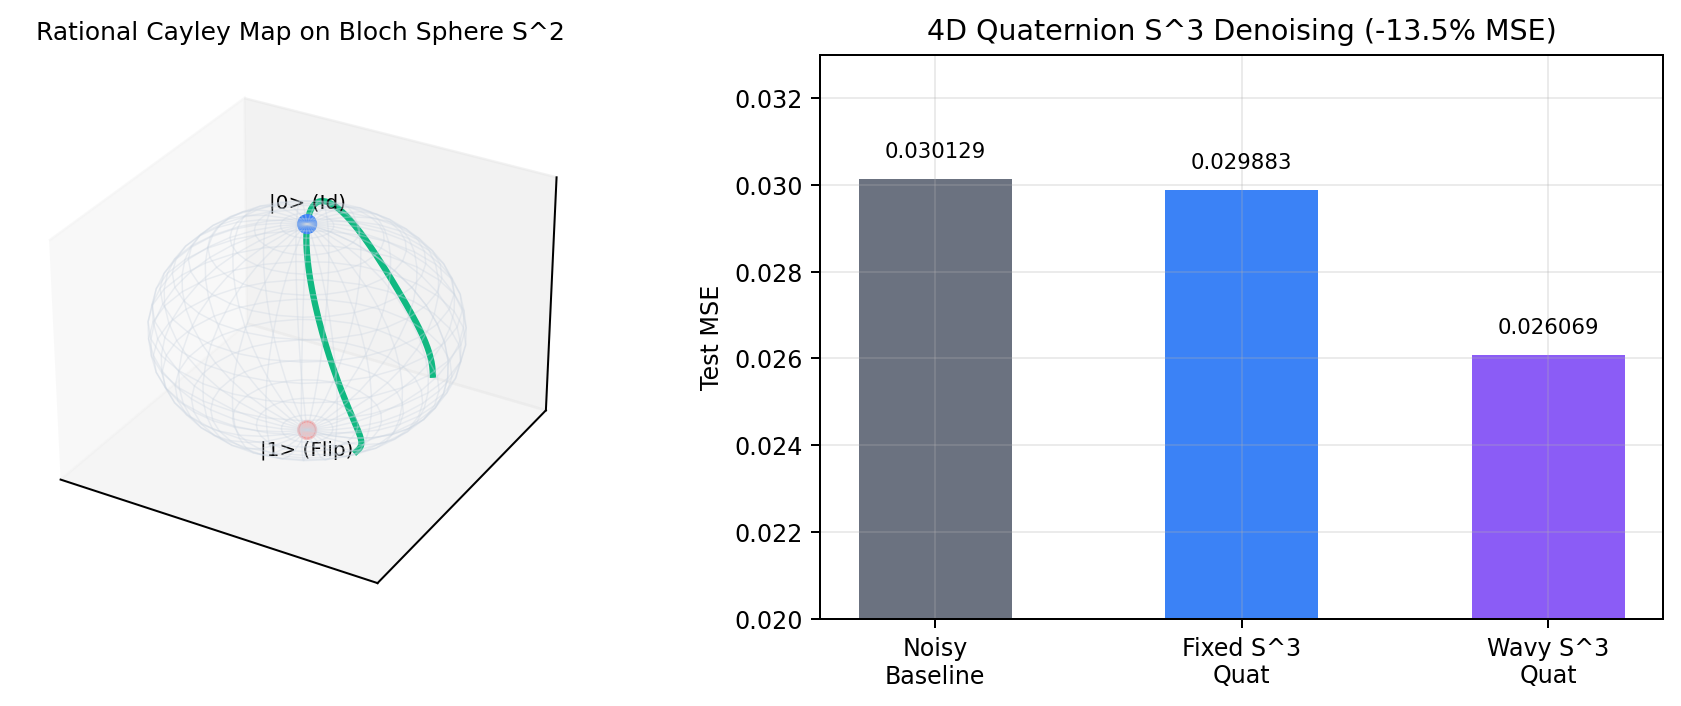
\includegraphics[width=\linewidth]{figures/fig7_bloch_sphere.png}
    \caption{Left: Rational Cayley $SU(2)$ trajectory on the 3D Bloch sphere $S^2$. Right: 4D quaternion $S^3$ denoising MSE.}
    \label{fig:bloch_s3}
\end{figure}

\section{The QM Atom Neuron and Rational Cayley Simplification}

\subsection{Schrödinger Orbital Neuron}
A 4-orbital quantum atom neuron evolves a ground state $|\psi_0\rangle = |1s\rangle \in \mathbb{C}^4$ under an input-perturbed Hermitian Hamiltonian:
\begin{equation}
    H(x) = H_0 + \sum_{j=1}^{d} x_j V_j, \quad |\psi(x)\rangle = e^{-iH(x)}|\psi_0\rangle,
\end{equation}
with Born expectation readout $\hat{y} = \langle \psi(x) | \hat{O} | \psi(x) \rangle \in \mathbb{R}$. Because $[V_1, V_2] \neq 0$, a \textbf{single} 4-orbital atom neuron (48 parameters, zero activation functions) solved 2D XOR to $0.00000000$ MSE in 150 Adam steps.

\subsection{Trig-Free Rational Cayley $SU(2)$ Derivation}
Exact \texttt{eigh} costs $\mathcal{O}(M^3)$. For $M=2$ (spin-$1/2$ Pauli atom), we replace $e^{-i\mathbf{h}\cdot\boldsymbol{\sigma}}$ with the unitary Cayley map:
\begin{equation}
    U(\mathbf{h}) = \frac{I - i\,\mathbf{h}\cdot\boldsymbol{\sigma}}{\sqrt{1 + \|\mathbf{h}\|^2}}, \qquad \mathbf{h} = \mathbf{h}_0 + V\mathbf{x} \in \mathbb{R}^3.
\end{equation}
Applying $U(\mathbf{h})$ to $|0\rangle = (1, 0)^\top$ yields $|\psi\rangle = \frac{1}{\sqrt{s}}(1 - ih_z,\; h_y - ih_x)^\top$ with $s = 1 + \|\mathbf{h}\|^2$. Computing $\mathbf{e} = \langle \psi | \boldsymbol{\sigma} | \psi \rangle$ cancels $\sqrt{s}$ completely:
\begin{equation}
\label{eq:cayley_bloch}
    \mathbf{e}(\mathbf{h}) = \frac{1}{1 + h_x^2 + h_y^2 + h_z^2}
    \begin{pmatrix}
        2(h_y + h_x h_z) \\
        2(-h_x + h_y h_z) \\
        1 + h_z^2 - h_x^2 - h_y^2
    \end{pmatrix}.
\end{equation}

\noindent\colorbox{tealbg}{\parbox{\dimexpr\columnwidth-2\fboxsep\relax}{%
\begin{proposition}
For all $\mathbf{h} \in \mathbb{R}^3$, $\|\mathbf{e}(\mathbf{h})\|_2 = 1$ identically, requiring zero \texttt{sqrt}, \texttt{sin}, or \texttt{cos} operations.
\end{proposition}
}}
\begin{proof}
Expanding the numerator squared sum gives $4(h_y + h_x h_z)^2 + 4(-h_x + h_y h_z)^2 + (1 + h_z^2 - h_x^2 - h_y^2)^2 = (1 + h_x^2 + h_y^2 + h_z^2)^2 = s^2$.
\end{proof}

On 2D XOR, \texttt{eigh} ($M=4$, 48p), \texttt{cayley} ($M=4$, 48p), and \texttt{su2\_pauli} ($M=2$, 13p) all achieved $0.00000000$ MSE, with vectorized \texttt{su2\_pauli} running 10,000 forward passes in $0.00647\text{ s}$ vs.\ $2.627\text{ s}$ (\texttt{eigh} loop). On 2.5-turn 2-spirals at exact parameter parity (193 params, 600 steps, Fig.~\ref{fig:xor_spirals}), \texttt{cayley\_su2\_fast} achieved $68.0\%$ test accuracy ($1.925\text{ s}$, $\max|\|\mathbf{e}\|-1| = 3.33\times 10^{-16}$) vs.\ $62.0\%$ for \texttt{real\_tanh\_mlp} ($0.862\text{ s}$) and $70.5\%$ for trig \texttt{su2\_spinor\_net} ($2.474\text{ s}$).

\begin{figure}[t]
    \centering
    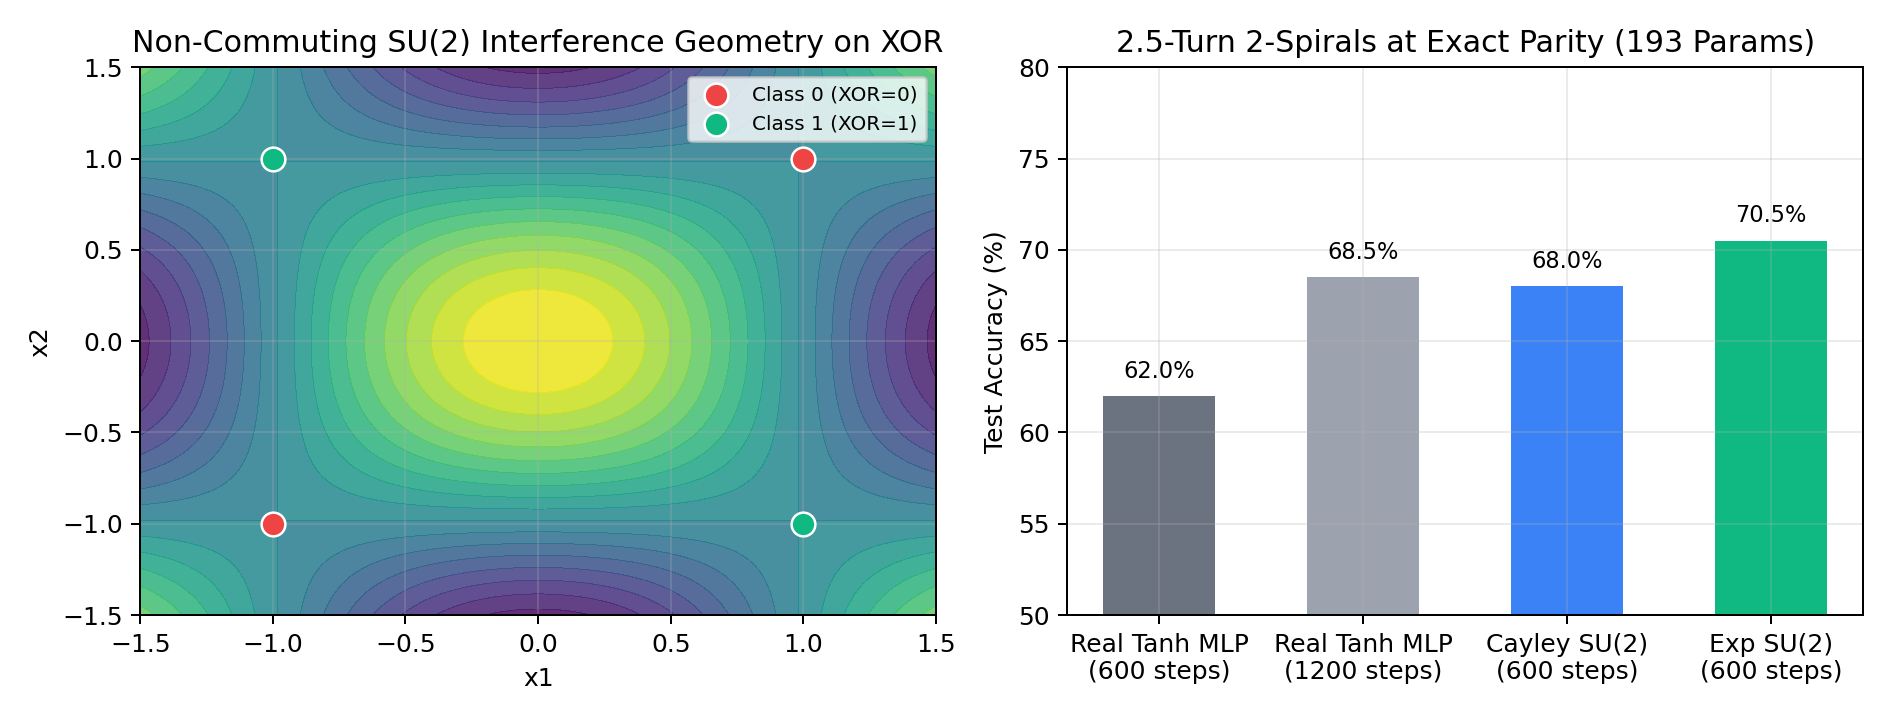
\includegraphics[width=\linewidth]{figures/fig3_qm_xor_spirals.png}
    \caption{Left: Non-commuting $SU(2)$ interference landscape on XOR. Right: 2.5-turn 2-spirals test accuracy at 193-parameter parity.}
    \label{fig:xor_spirals}
\end{figure}

\section{QuatScan: Non-Abelian Sequence Memory}
Using the rational Cayley map, each token $v$ emits a unit quaternion $u_t = (1, -\mathbf{h}_t) / \sqrt{1 + \|\mathbf{h}_t\|^2} \in S^3$, updating an associative sequence state without positional encodings:
\begin{equation}
    q_t = u_t \otimes q_{t-1}, \qquad q_0 = (1, 0, 0, 0).
\end{equation}
Because quaternion multiplication is associative, $q_t$ is computable in an $\mathcal{O}(\log L)$ parallel prefix scan; because it is non-commutative, $u_A \otimes u_B \neq u_B \otimes u_A$.

We tested this on an order-sensitive sequence task ($L=16$, 4 tokens $\{A,B,C,D\}$, label $1$ iff $\text{pos}(A) < \text{pos}(B)$, zero positional encodings). Commutative $U(1)$ memory is mathematically blind to order and scored $53.5\%$ (49 params). With standard $\mathcal{N}(0, 1)$ initialization, 14 random $C/D$ distractors scrambled $q_t$ into a random walk on $S^3$ ($51.0\%$). Switching to near-identity initialization ($\sigma_{\text{init}} = 0.1$) resolved the random-walk bottleneck immediately: \texttt{su2\_quat\_memory} (65 params, zero \texttt{ReLU}/\texttt{tanh}, zero trig) reached \textbf{100.0\% test accuracy} with $\max||q_T|-1| = 1.55\times 10^{-15}$ (Fig.~\ref{fig:quatscan}).

\begin{figure}[t]
    \centering
    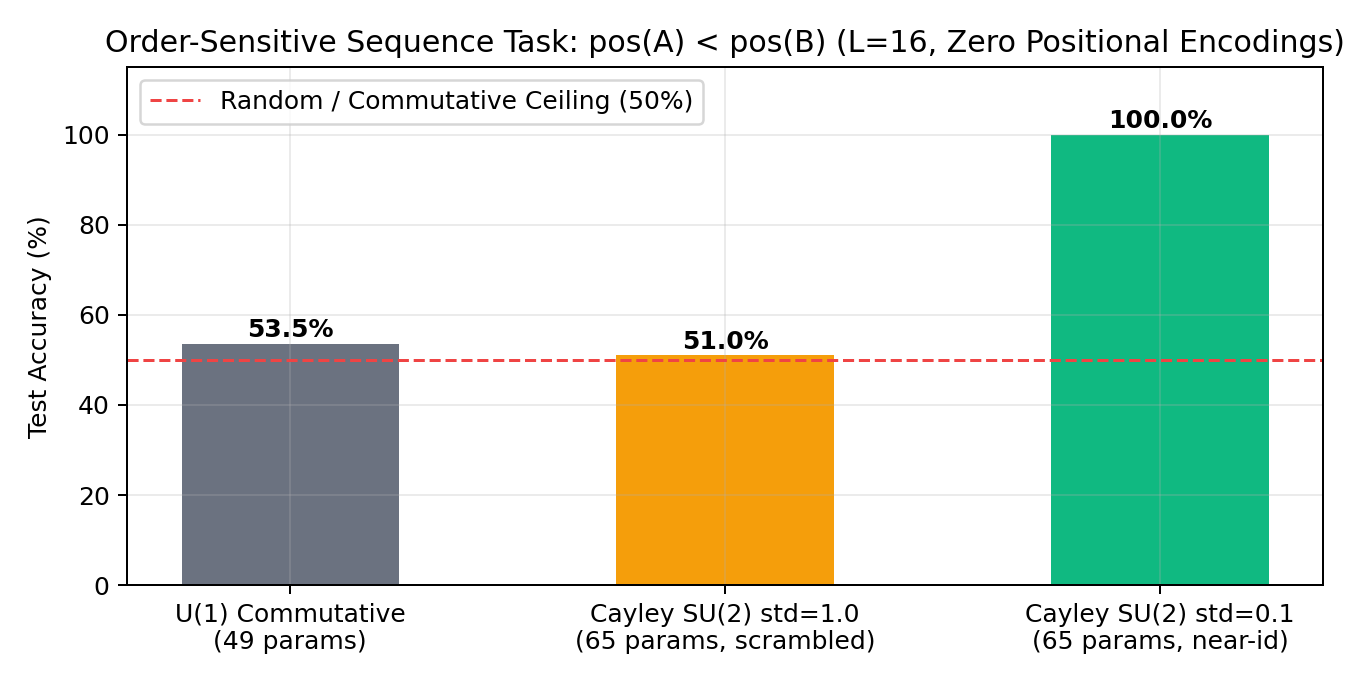
\includegraphics[width=\linewidth]{figures/fig4_quatscan_order.png}
    \caption{Order-sensitive sequence accuracy ($L=16$, zero positional encodings): commutative $U(1)$ is stuck near $50\%$, while near-identity Cayley $SU(2)$ reaches $100.0\%$.}
    \label{fig:quatscan}
\end{figure}

\section{Limitations and Future Work}
\begin{itemize}
    \item \textbf{Unfused NumPy overhead:} Even without trig, \texttt{cayley\_su2\_fast} is $\approx 2.2\times$ slower than BLAS \texttt{matmul + tanh} in unfused NumPy due to elementwise array temporaries; a fused CUDA/Triton kernel is needed to realize its theoretical speed.
    \item \textbf{Initialization sensitivity:} Non-abelian $S^3$ scans require near-identity initialization ($\sigma_{\text{init}} \ll 1$) on long sequences to avoid random-walk scrambling.
    \item \textbf{Multi-layer scale:} Testing \texttt{QuatScan} on long-range real-world benchmarks (e.g., Long Range Arena or language modeling) remains open.
\end{itemize}

\end{document}
